\subsection{GPR Results}

\lorena{Using GPR to create a map between the injected and recovered masses and
spins of the O2 dataset allows us to better predict the instrisic parameters of 
a binary system. Fig~\ref{m_chi_comparisons} shows the predictions from the O2 
testing dataset. The gray circles represent the recovered values from the 
best-fit template, the orange circles are the predictions coming from regression, 
and the true values are depicted by the black line. Ideally, all values would lie 
along the line.}

\begin{table}
  \caption{\label{tab:NN_errors}  Mean differences in absolute value 
    $|\Delta \bar{y}|=  \frac{1}{N} \Sigma |y^i_{\rm inj} - y^i_{\rm rec/pred}|$
    and averages of the relative differences in absolute value 
    $|\delta \bar{y}| = \frac{1}{N} \Sigma \left( |y^i_{\rm inj} - 
    y^i_{\rm rec/pred}|/y^i_{\rm inj} \right) $ for recovered and predicted data.
    For spin variables, the standard deviation $\sigma_y$ is computed from the 
    former, while for mass variables is computed from the latter. Note that 
    ${\cal{M}}_c$ is not predicted by the NN but it is computed from the 
    predicted $m_i$.}
  \begin{center}
  \begin{tabular}{c|ccc|ccc}
  \hline\hline
  & $|\Delta \bar{y}_{\rm rec}|$  & $|\delta \bar{y}_{\rm rec}|$  & $\sigma_y^{\rm rec}$ &
     $|\Delta \bar{y}_{\rm pred}|$ & $|\delta \bar{y}_{\rm pred}|$ & $\sigma_y^{\rm pred}$ \\
  \hline\hline
$m_1$          & $6.625$ & $0.352$ & $0.596$ & $3.241$ & $0.127$ & $0.305$ \\
$m_2$          & $2.761$ & $0.256$ & $0.351$ & $1.414$ & $0.111$ & $0.337$ \\
$\chi_1$       & $0.266$ &  /  & $0.388$ & $0.134$ &  /  & $0.194$ \\
$\chi_2$       & $0.277$ &  /  & $0.460$ & $0.151$ &  /  & $0.225$ \\
\hline
${\cal{M}}_c$  & $1.323$ & $0.039$ & $0.104$ & $0.712$ & $0.027$ & $0.079$ \\
  \hline\hline
  \end{tabular}
  \end{center}
\end{table}

\begin{table}
  \caption{\label{tab:NN_errors_temp} As Table~\ref{tab:NN_errors} but predicting $(m_1, {\cal{M}}_c, \chi_1, \chi_2)$. }
  \begin{center}
  \begin{tabular}{c|ccc|ccc}
  \hline\hline
 %& $\bar{|\Delta y_{\rm rec}|}$ & $\bar{|\Delta y_{\rm rec}/y|}$ & $\bar{|\sigma_y_{\rm rec}|}$ & & &  \\
  & $|\Delta \bar{y}_{\rm rec}|$  & $|\delta \bar{y}_{\rm rec}|$  & $\sigma_y^{\rm rec}$ & 
     $|\Delta \bar{y}_{\rm pred}|$ & $|\delta \bar{y}_{\rm pred}|$ & $\sigma_y^{\rm pred}$ \\
  \hline\hline
$m_1$          & $6.625$ & $0.352$ & $0.596$ & $3.247$ & $0.127$ & $0.302$ \\
${\cal{M}}_c$  & $1.323$ & $0.039$ & $0.104$ & $0.704$ & $0.027$ & $0.090$ \\
$\chi_1$       & $0.266$ &  /  & $0.388$ & $0.135$ &  /  & $0.193$ \\
$\chi_2$       & $0.277$ &  /  & $0.460$ & $0.150$ &  /  & $0.225$ \\
\hline
$m_2$          & $2.761$ & $0.256$ & $0.351$ & $1.407$ & $0.114$ & $0.350$ \\
  \hline\hline
  \end{tabular}
  \end{center}
\end{table}

%The difference between the recovered and predicted values is 
%clear especially in cases when the recovered masses are very high.  
%Similarly, in Fig.~\ref{m_chi1_chi2_comparisons} the 
%primary spins are closer to the true value using regression. Regression also
%gets rid of highly negative and positive secondary spins that are far from the
%true values. Although both the recovered and the predicted values have seemingly 
%large errors, the predictions improve the overall error significantly.}

\begin{figure}
    \centering
    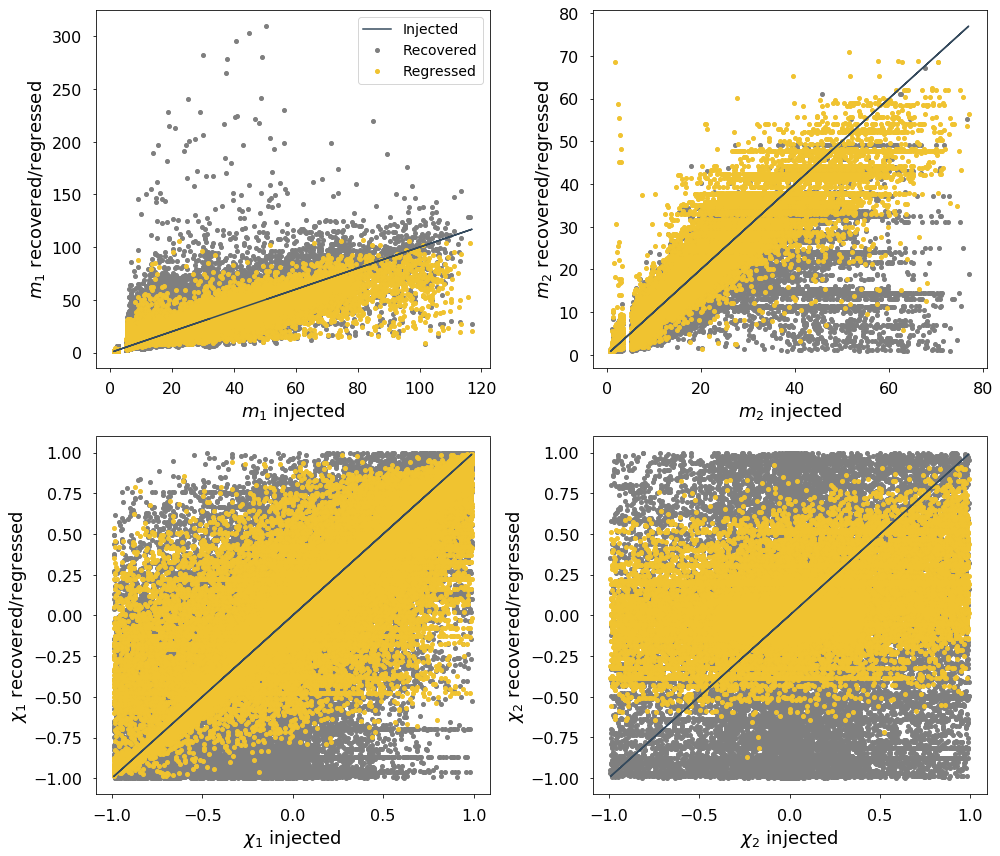
\includegraphics[width=0.45\textwidth]{m_chi_comparisons.png}
    \caption{The top panels show the recovered (gray) and regressed (orange)
             masses as a function of the injected values. The bottom panels 
             show the same functions for the spin magnitudes. The black line 
             denotes a perfect recovery and regression.
            }
        \label{m_chi_comparisons}
\end{figure}

\begin{figure}
    \centering
    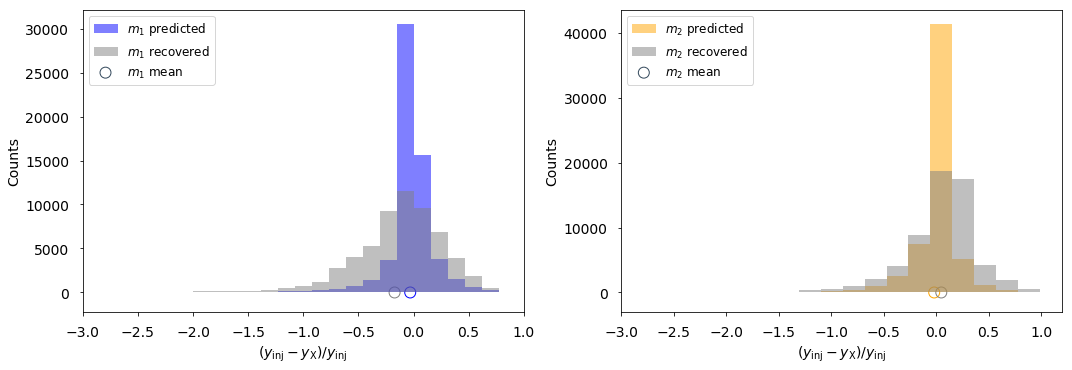
\includegraphics[width=0.45\textwidth]{m1_m2_chi_error_analysis_wboxes.png}
    \caption{The top panels show the distributions of the mean relative errors 
            for the recovered (gray) and regressed (orange) masses. The bottom
            panels show the distributions of the mean difference for the spins
            magnitudes.
            }
        \label{m_chi_comparisons}
\end{figure}

\lorena{To quantify the above...}
